\documentclass{beamer}
\usepackage[utf8]{inputenc}
\usepackage{graphicx, epsfig}
\usepackage{amsmath,mathrsfs,amsfonts,amssymb}
\usepackage{floatflt}
\usepackage{epic,ecltree}
\usepackage{mathtext}
\usepackage{fancybox}
\usepackage{fancyhdr}
\usepackage{multirow}
\usepackage{enumerate}
\usepackage{epstopdf}
\usepackage{multicol}
\usepackage{algorithm}
\usepackage[noend]{algorithmic}
\usepackage{tikz}
\usepackage{blindtext}
\usetheme{default}%{Singapore}%{Warsaw}%{Warsaw}%{Darmstadt}
\usecolortheme{default}

\setbeamerfont{title}{size=\Huge}
\setbeamertemplate{footline}[page number]{}

\setbeamertemplate{section in toc}[sections numbered]


\makeatletter
\newcommand\HUGE{\@setfontsize\Huge{35}{40}}
\makeatother    

\setbeamerfont{title}{size=\HUGE}
\beamertemplatenavigationsymbolsempty

% latin bold lower
\newcommand{\ba}{\mathbf{a}} 
\newcommand{\bc}{\mathbf{c}} 
\newcommand{\be}{\mathbf{e}} 
\newcommand{\bh}{\mathbf{h}} 
\newcommand{\bp}{\mathbf{p}} 
\newcommand{\bt}{\mathbf{t}} 
\newcommand{\bs}{\mathbf{s}} 
\newcommand{\bu}{\mathbf{u}} 
\newcommand{\bv}{\mathbf{v}} 
\newcommand{\bw}{\mathbf{w}} 
\newcommand{\bx}{\mathbf{x}} 
\newcommand{\by}{\mathbf{y}} 
\newcommand{\bz}{\mathbf{z}} 

% latin bold upper
\newcommand{\bA}{\mathbf{A}} 
\newcommand{\bB}{\mathbf{B}} 
\newcommand{\bC}{\mathbf{C}} 
\newcommand{\bI}{\mathbf{I}} 
\newcommand{\bL}{\mathbf{L}} 
\newcommand{\bM}{\mathbf{M}} 
\newcommand{\bQ}{\mathbf{Q}} 
\newcommand{\bT}{\mathbf{T}} 
\newcommand{\bU}{\mathbf{U}} 
\newcommand{\bV}{\mathbf{V}} 
\newcommand{\bW}{\mathbf{W}} 
\newcommand{\bX}{\mathbf{X}} 
\newcommand{\bY}{\mathbf{Y}} 
\newcommand{\bZ}{\mathbf{Z}} 

% latin cal upper
\newcommand{\cG}{\mathcal{G}} 
\newcommand{\cL}{\mathcal{L}} 
\newcommand{\cN}{\mathcal{N}} 
\newcommand{\cS}{\mathcal{S}} 
\newcommand{\cT}{\mathcal{T}} 
\newcommand{\cW}{\mathcal{W}} 
\newcommand{\cX}{\mathcal{X}} 
\newcommand{\cZ}{\mathcal{Z}} 

% latin bb upper
\newcommand{\bbE}{\mathbb{E}} 
\newcommand{\bbI}{\mathbb{I}} 
\newcommand{\bbP}{\mathbb{P}} 
\newcommand{\bbR}{\mathbb{R}} 

% greek bold lower
\newcommand{\bepsilon}{\boldsymbol{\epsilon}} 
\newcommand{\btheta}{\boldsymbol{\theta}} 
\newcommand{\blambda}{\boldsymbol{\lambda}} 
\newcommand{\bpi}{\boldsymbol{\pi}} 
\newcommand{\bmu}{\boldsymbol{\mu}} 
\newcommand{\bsigma}{\boldsymbol{\sigma}} 
\newcommand{\bphi}{\boldsymbol{\phi}} 

% greek bold upper
\newcommand{\bSigma}{\boldsymbol{\Sigma}} 

\DeclareMathOperator*{\argmin}{arg\,min}
\DeclareMathOperator*{\argmax}{arg\,max}

\newcommand{\createdgmtitle}[1]{\title[\hbox to 56mm{Deep Generative Models  \hfill\insertframenumber\,/\,\inserttotalframenumber}]
	{Deep Generative Models \\ {\Huge Lecture #1}}
	\author{Roman Isachenko}
	\institute{
\includegraphics[width=0.5cm]{../utils/ozonmasterslogo} \large{Ozon Masters}}
	\date{Spring, 2022}
}

\newcommand\myfootnote[1]{%
  \tikz[remember picture,overlay]
  \draw (current page.south west) +(1in + \oddsidemargin,0.5em)
  node[anchor=south west,inner sep=0pt]{\parbox{\textwidth}{%
      \rlap{\rule{10em}{0.4pt}}\raggedright\scriptsize \textit{#1}}};}

\newcommand\myfootnotewithlink[2]{%
  \tikz[remember picture,overlay]
  \draw (current page.south west) +(1in + \oddsidemargin,0.5em)
  node[anchor=south west,inner sep=0pt]{\parbox{\textwidth}{%
      \rlap{\rule{10em}{0.4pt}}\raggedright\scriptsize\href{#1}{\textit{#2}}}};}
      
\AtBeginSection[]
{
	\begin{frame}{Outline}
		\tableofcontents[currentsection,subsectionstyle=hide]
	\end{frame}
}
\AtBeginSubsection[]{
	\begin{frame}{Outline}
		\tableofcontents[currentsection,currentsubsection]
	\end{frame}
}
\createdgmtitle{5}

\usepackage{tikz}

\usetikzlibrary{arrows,shapes,positioning,shadows,trees}
%--------------------------------------------------------------------------------
\begin{document}
%--------------------------------------------------------------------------------
\begin{frame}[noframenumbering,plain]
%\thispagestyle{empty}
\titlepage
\end{frame}
%=======
\begin{frame}{Recap of previous lecture}
	\begin{minipage}[t]{0.55\columnwidth}
		\begin{block}{Variational autoencoder (VAE)}
		    \begin{itemize}
			    \item VAE learns stochastic mapping between $\bx$-space, from $\pi(\bx)$, and a latent $\bz$-space, with simple distribution. 
			    \item The generative model learns  distribution $p(\bx, \bz | \btheta) = p(\bz) p(\bx |\bz, \btheta)$, with a prior distribution $p(\bz)$, and a stochastic decoder $p(\bx|\bz, \btheta)$. 
			    \item The stochastic encoder $q(\bz|\bx, \bphi)$ (inference model), approximates the true but intractable posterior $p(\bz|\bx, \btheta)$.
		    \end{itemize}
	    \end{block}
	\end{minipage}%
	\begin{minipage}[t]{0.45\columnwidth}
		\vspace{0.7cm}
		\begin{figure}[h]
			\centering
			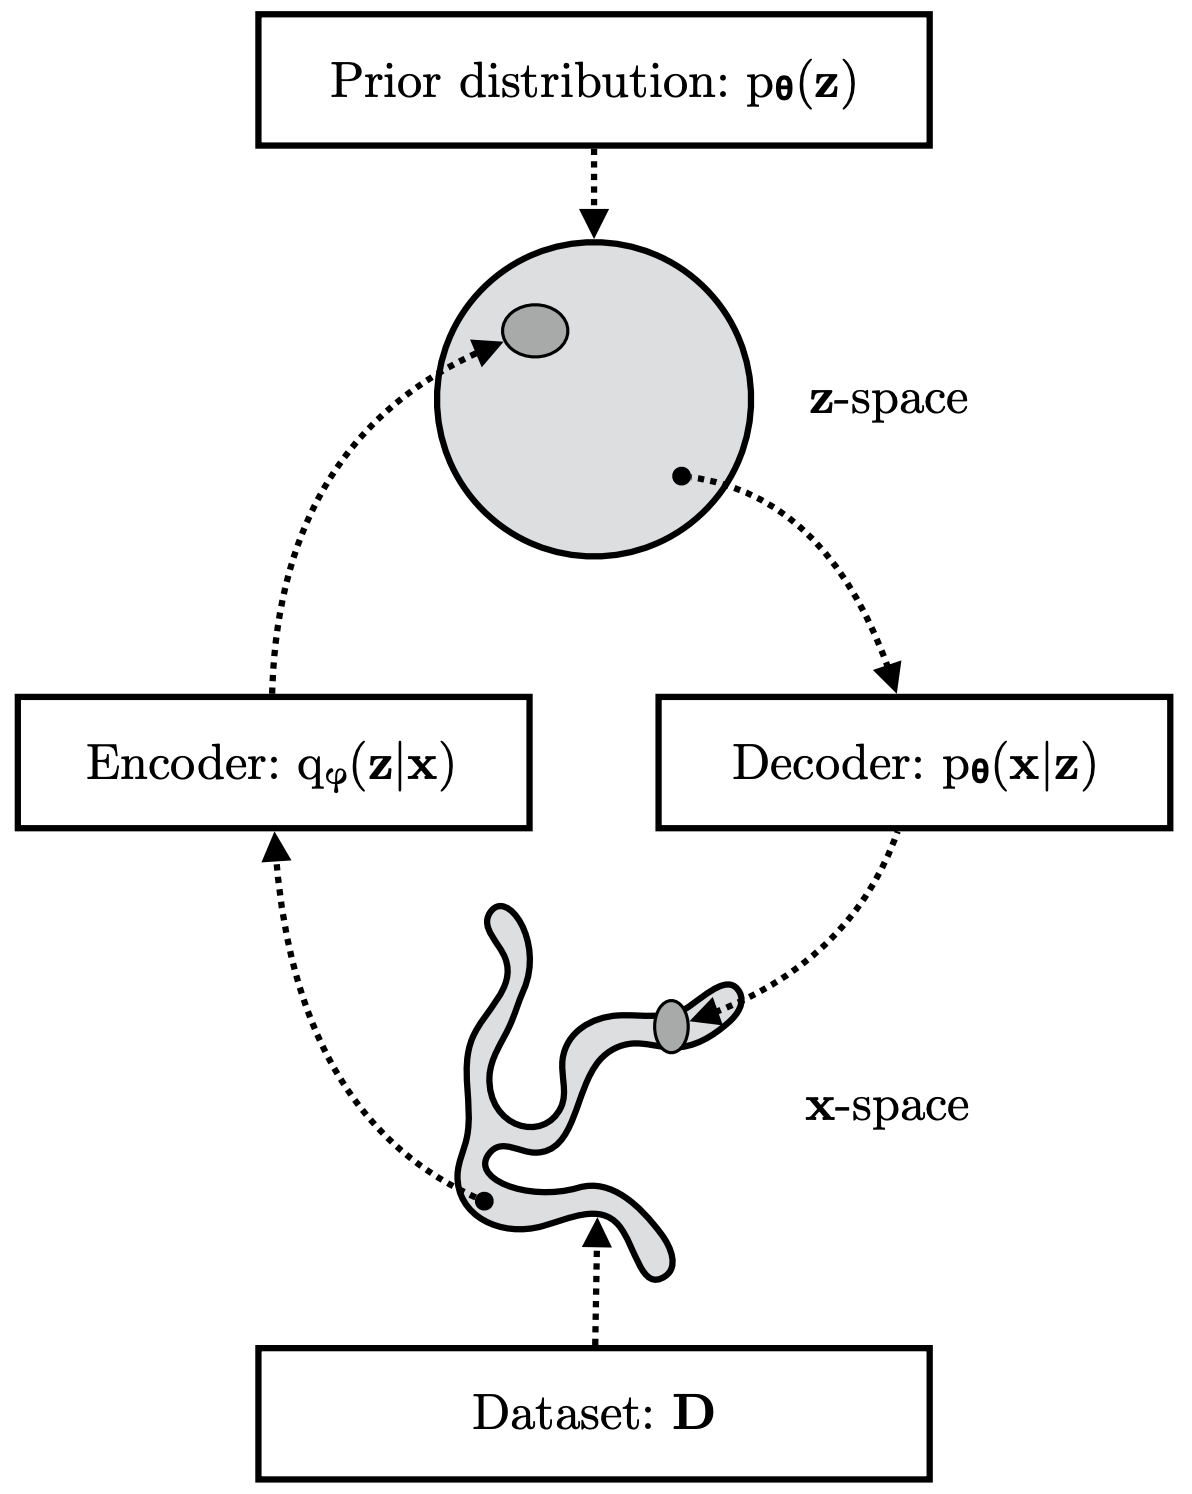
\includegraphics[width=\linewidth]{figs/vae_scheme}
		\end{figure}
	\end{minipage}
	
	\myfootnotewithlink{https://arxiv.org/abs/1906.02691}{Kingma D. P., Welling M. An introduction to variational autoencoders, 2019}
\end{frame}
%=======
\begin{frame}{Recap of previous lecture}
	\begin{block}{LVM}
		\vspace{-0.3cm}
		\[
		    p(\bx | \btheta) = \int p(\bx, \bz | \btheta) d \bz = \int p(\bx | \bz, \btheta) p(\bz) d \bz 
		\]
		\vspace{-0.3cm}
	\end{block}
	\begin{itemize}
		\item More powerful $p(\bx | \bz, \btheta)$ leads to more powerful generative model $p(\bx | \btheta)$.
		\item Too powerful $p(\bx | \bz, \btheta)$ could lead to posterior collapse: $q(\bz | \bx)$ will not carry any information about $\bx$ and close to prior $p(\bz)$.
	\end{itemize}
	\begin{block}{Autoregressive decoder}
		\vspace{-0.2cm}
		\[
		    p(\bx | \bz , \btheta) = \prod_{i=1}^n p(x_i | \bx_{1:i - 1}, \bz , \btheta)
		\]
	\end{block}
	\begin{itemize}
		\item Global structure is captured by latent variables.
		\item Local statistics are captured by limited receptive field autoregressive model.
	\end{itemize}
	
	\myfootnotewithlink{https://arxiv.org/abs/1611.05013}{Gulrajani I. et al. PixelVAE: A Latent Variable Model for Natural Images, 2016}
\end{frame}
%=======
\begin{frame}{Recap of previous lecture}
	\begin{block}{Decoder weakening}
		\begin{itemize}
			\item Powerful decoder $p(\bx | \bz, \btheta)$ makes the model expressive, but posterior collapse is possible.
			\item PixelVAE model uses the autoregressive PixelCNN model with small number of layers to limit receptive field.
		\end{itemize}
	\end{block}
	
	\begin{block}{KL annealing}
		\vspace{-0.2cm}
		\[
		    \mathcal{L}(q, \btheta, \beta) = \mathbb{E}_{q(\bz | \bx)} \log p(\bx | \bz, \btheta) - \beta \cdot KL (q(\bz | \bx) || p(\bz))
		\]
		Start training with $\beta = 0$, increase it until $\beta = 1$ during training.
	\end{block}
	
	\begin{block}{Free bits}
		Ensure the use of less than $\lambda$ bits of information:
		\[
		    \mathcal{L}(q, \btheta, \lambda) = \mathbb{E}_{q(\bz | \bx)} \log p(\bx | \bz, \btheta) - \max(\lambda, KL (q(\bz | \bx) || p(\bz))).
		\]
		This results in $KL (q(\bz | \bx) || p(\bz)) \geq \lambda$.
	\end{block}
\end{frame}
%=======
\begin{frame}{Recap of previous lecture}
	\begin{block}{VAE objective}
		\vspace{-0.2cm}
		\[
		\log p(\bx | \btheta) \geq \mathcal{L} (q, \btheta)  = \mathbb{E}_{q(\bz | \bx)} \log \frac{p(\bx, \bz | \btheta)}{q(\bz| \bx)} \rightarrow \max_{q, \btheta}
		\]
		\vspace{-0.2cm}
	\end{block}
	\begin{block}{IWAE objective}
		\vspace{-0.4cm}
		\[
		\mathcal{L}_K (q, \btheta)  = \mathbb{E}_{\bz_1, \dots, \bz_K \sim q(\bz | \bx)} \log \left( \frac{1}{K}\sum_{k=1}^K\frac{p(\bx, \bz_k | \btheta)}{q(\bz_k| \bx)} \right) \rightarrow \max_{q, \btheta}.
		\]
		\vspace{-0.4cm}
	\end{block}
	\begin{block}{Theorem}
		\begin{enumerate}
			\item $\log p(\bx | \btheta) \geq \mathcal{L}_K (q, \btheta) \geq \mathcal{L}_M (q, \btheta) \geq \mathcal{L} (q, \btheta), \quad \text{for } K \geq M$;
			\item $\log p(\bx | \btheta) = \lim_{K \rightarrow \infty} \mathcal{L}_K (q, \btheta)$ if $\frac{p(\bx, \bz | \btheta)}{q(\bz | \bx)}$ is bounded.
		\end{enumerate}
	\end{block}
	\myfootnotewithlink{https://arxiv.org/abs/1509.00519}{Burda Y., Grosse R., Salakhutdinov R. Importance Weighted Autoencoders, 2015}
\end{frame}
%=======
\begin{frame}{Outline}
	\tableofcontents
\end{frame}
\AtBeginSection[ ]
{
	\begin{frame}{Outline}
		\tableofcontents[currentsection]
	\end{frame}
}
%=======
\begin{frame}{Likelihood-based models so far...}
	\begin{minipage}[t]{0.5\columnwidth}
		\begin{block}{Autoregressive models}
			\vspace{-0.5cm}
			\[
				p(\bx|\btheta) = \prod_{i=1}^m p(x_i | \bx_{1:i - 1}, \btheta)
			\]
			\vspace{-0.2cm}
			\begin{itemize}
				\item tractable likelihood, 
				\item no inferred latent factors.
			\end{itemize}
		\end{block}
	\end{minipage}%
	\begin{minipage}[t]{0.5\columnwidth}
		\begin{block}{Latent variable models}
			\[
				p(\bx| \btheta) = \int p(\bx, \bz | \btheta) d \bz
			\]
			\begin{itemize}
				\item latent feature representation, 
				\item intractable likelihood.
			\end{itemize}
		\end{block}
	\end{minipage}
	
	\vspace{1cm } 
	How to build model with latent variables and tractable likelihood?
\end{frame}
%=======
\begin{frame}{Generative models zoo}
	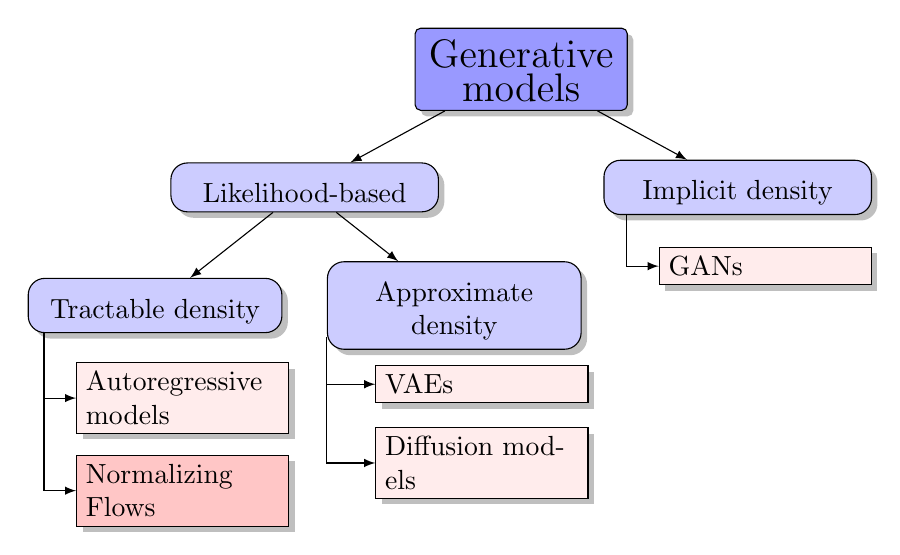
\begin{tikzpicture}[
	 	basic/.style  = {draw, text width=2cm, drop shadow, rectangle},
	 	root/.style   = {basic, rounded corners=2pt, thin, text height=1.1em, text width=7em, align=center, fill=blue!40},
	 	level 1/.style={sibling distance=55mm},
	 	level 2/.style = {basic, rounded corners=6pt, thin, align=center, fill=blue!20, text height=1.1em, text width=9em, sibling distance=38mm},
	 	level 3/.style = {basic, rounded corners=6pt, thin,align=center, fill=blue!20, text width=8.5em},
	 	level 4/.style = {basic, thin, align=left, fill=pink!30, text width=7em},
	 	level 5/.style = {basic, thin, align=left, fill=pink!90, text width=7em},
		edge from parent/.style={->,draw},
		>=latex]
		
		% root of the the initial tree, level 1
		\node[root] {\Large Generative models}
		% The first level, as children of the initial tree
		child {node[level 2] (c1) {Likelihood-based}
			child {node[level 3] (c11) {Tractable density}}
			child {node[level 3] (c12) {Approximate density}}
		}
		child {node[level 2] (c2) {Implicit density}};
		
		% The second level, relatively positioned nodes
		\begin{scope}[every node/.style={level 4}]
		\node [below of = c11, yshift=-5pt, xshift=10pt] (c111) {Autoregressive models};
		
		\node [below of = c12, xshift=10pt] (c121) {VAEs};
		\node [below of = c121] (c122) {Diffusion models};
		\node [below of = c2, xshift=10pt] (c21) {GANs};
		
		\end{scope}
		
		% The second level, relatively positioned nodes
		\begin{scope}[every node/.style={level 5}]
			\node [below of = c111, yshift=-5pt] (c112) {Normalizing Flows};
		\end{scope}
		
		
		% lines from each level 1 node to every one of its "children"
		\foreach \value in {1,2}
		\draw[->] (c11.194) |- (c11\value.west);
		
		\foreach \value in {1,2}
		\draw[->] (c12.194) |- (c12\value.west);
		
		\draw[->] (c2.194) |- (c21.west);
		
	\end{tikzpicture}
\end{frame}
%=======
\begin{frame}{Normalizing flows prerequisites}
	\begin{block}{Change of variable theorem}
		Let $\bx$ be a random variable with density function $p(\bx)$ and $f: \mathbb{R}^m \rightarrow \mathbb{R}^m$ is a differentiable, invertible function (diffeomorphism). If $\bz = f(\bx)$, $\bx = f^{-1}(\bz) = g(\bz)$, then
		\begin{align*}
			p(\bx) &= p(\bz) \left|\det \left(  \frac{\partial \bz}{\partial \bx} \right) \right| = p(f(\bx)) \left|\det \left(  \frac{\partial f(\bx)}{\partial \bx} \right) \right| \\
			p(\bz) &= p(\bx) \left|\det \left(  \frac{\partial \bx}{\partial \bz} \right) \right| = p(g(\bz)) \left|\det \left(  \frac{\partial g(\bz)}{\partial \bz} \right) \right|.
		\end{align*}
		\vspace{-0.5cm}
	\end{block}
	\begin{block}{Inverse function theorem}
		If function $f$ is invertible and Jacobian is continuous and non-singular, then
		\[
			\left|\det \left(  \frac{\partial f(\bx)}{\partial \bx} \right)\right| = \left|\det \left(  \frac{\partial g^{-1}(\bx)}{\partial \bx} \right)\right| = \left|\det \left(  \frac{\partial g(\bz)}{\partial \bz} \right)\right|^{-1}
		\]
	\end{block}
\end{frame}
%=======
\begin{frame}{Jacobian-determinant}
	\[
		p(\bx | \btheta) = p(f(\bx, \btheta)) \left|\det \left(  \frac{\partial f(\bx,\btheta)}{\partial \bx} \right) \right| 
	\]
	\begin{minipage}{0.55\columnwidth}
		\begin{itemize}
			\item $\bx$ and $\bz$ have the same dimensionality ($\bbR^m$).
			\vfill
			\item $f(\bx, \btheta)$ could be parametric function.
			\vfill
			\item Determinant of Jacobian $\mathbf{J} =\frac{\partial f(\bx, \btheta)}{\partial \bx}$ shows how the volume changes under the transorfmation.
		\end{itemize}
	\end{minipage}%
	\begin{minipage}{0.45\columnwidth}
		\begin{figure}
			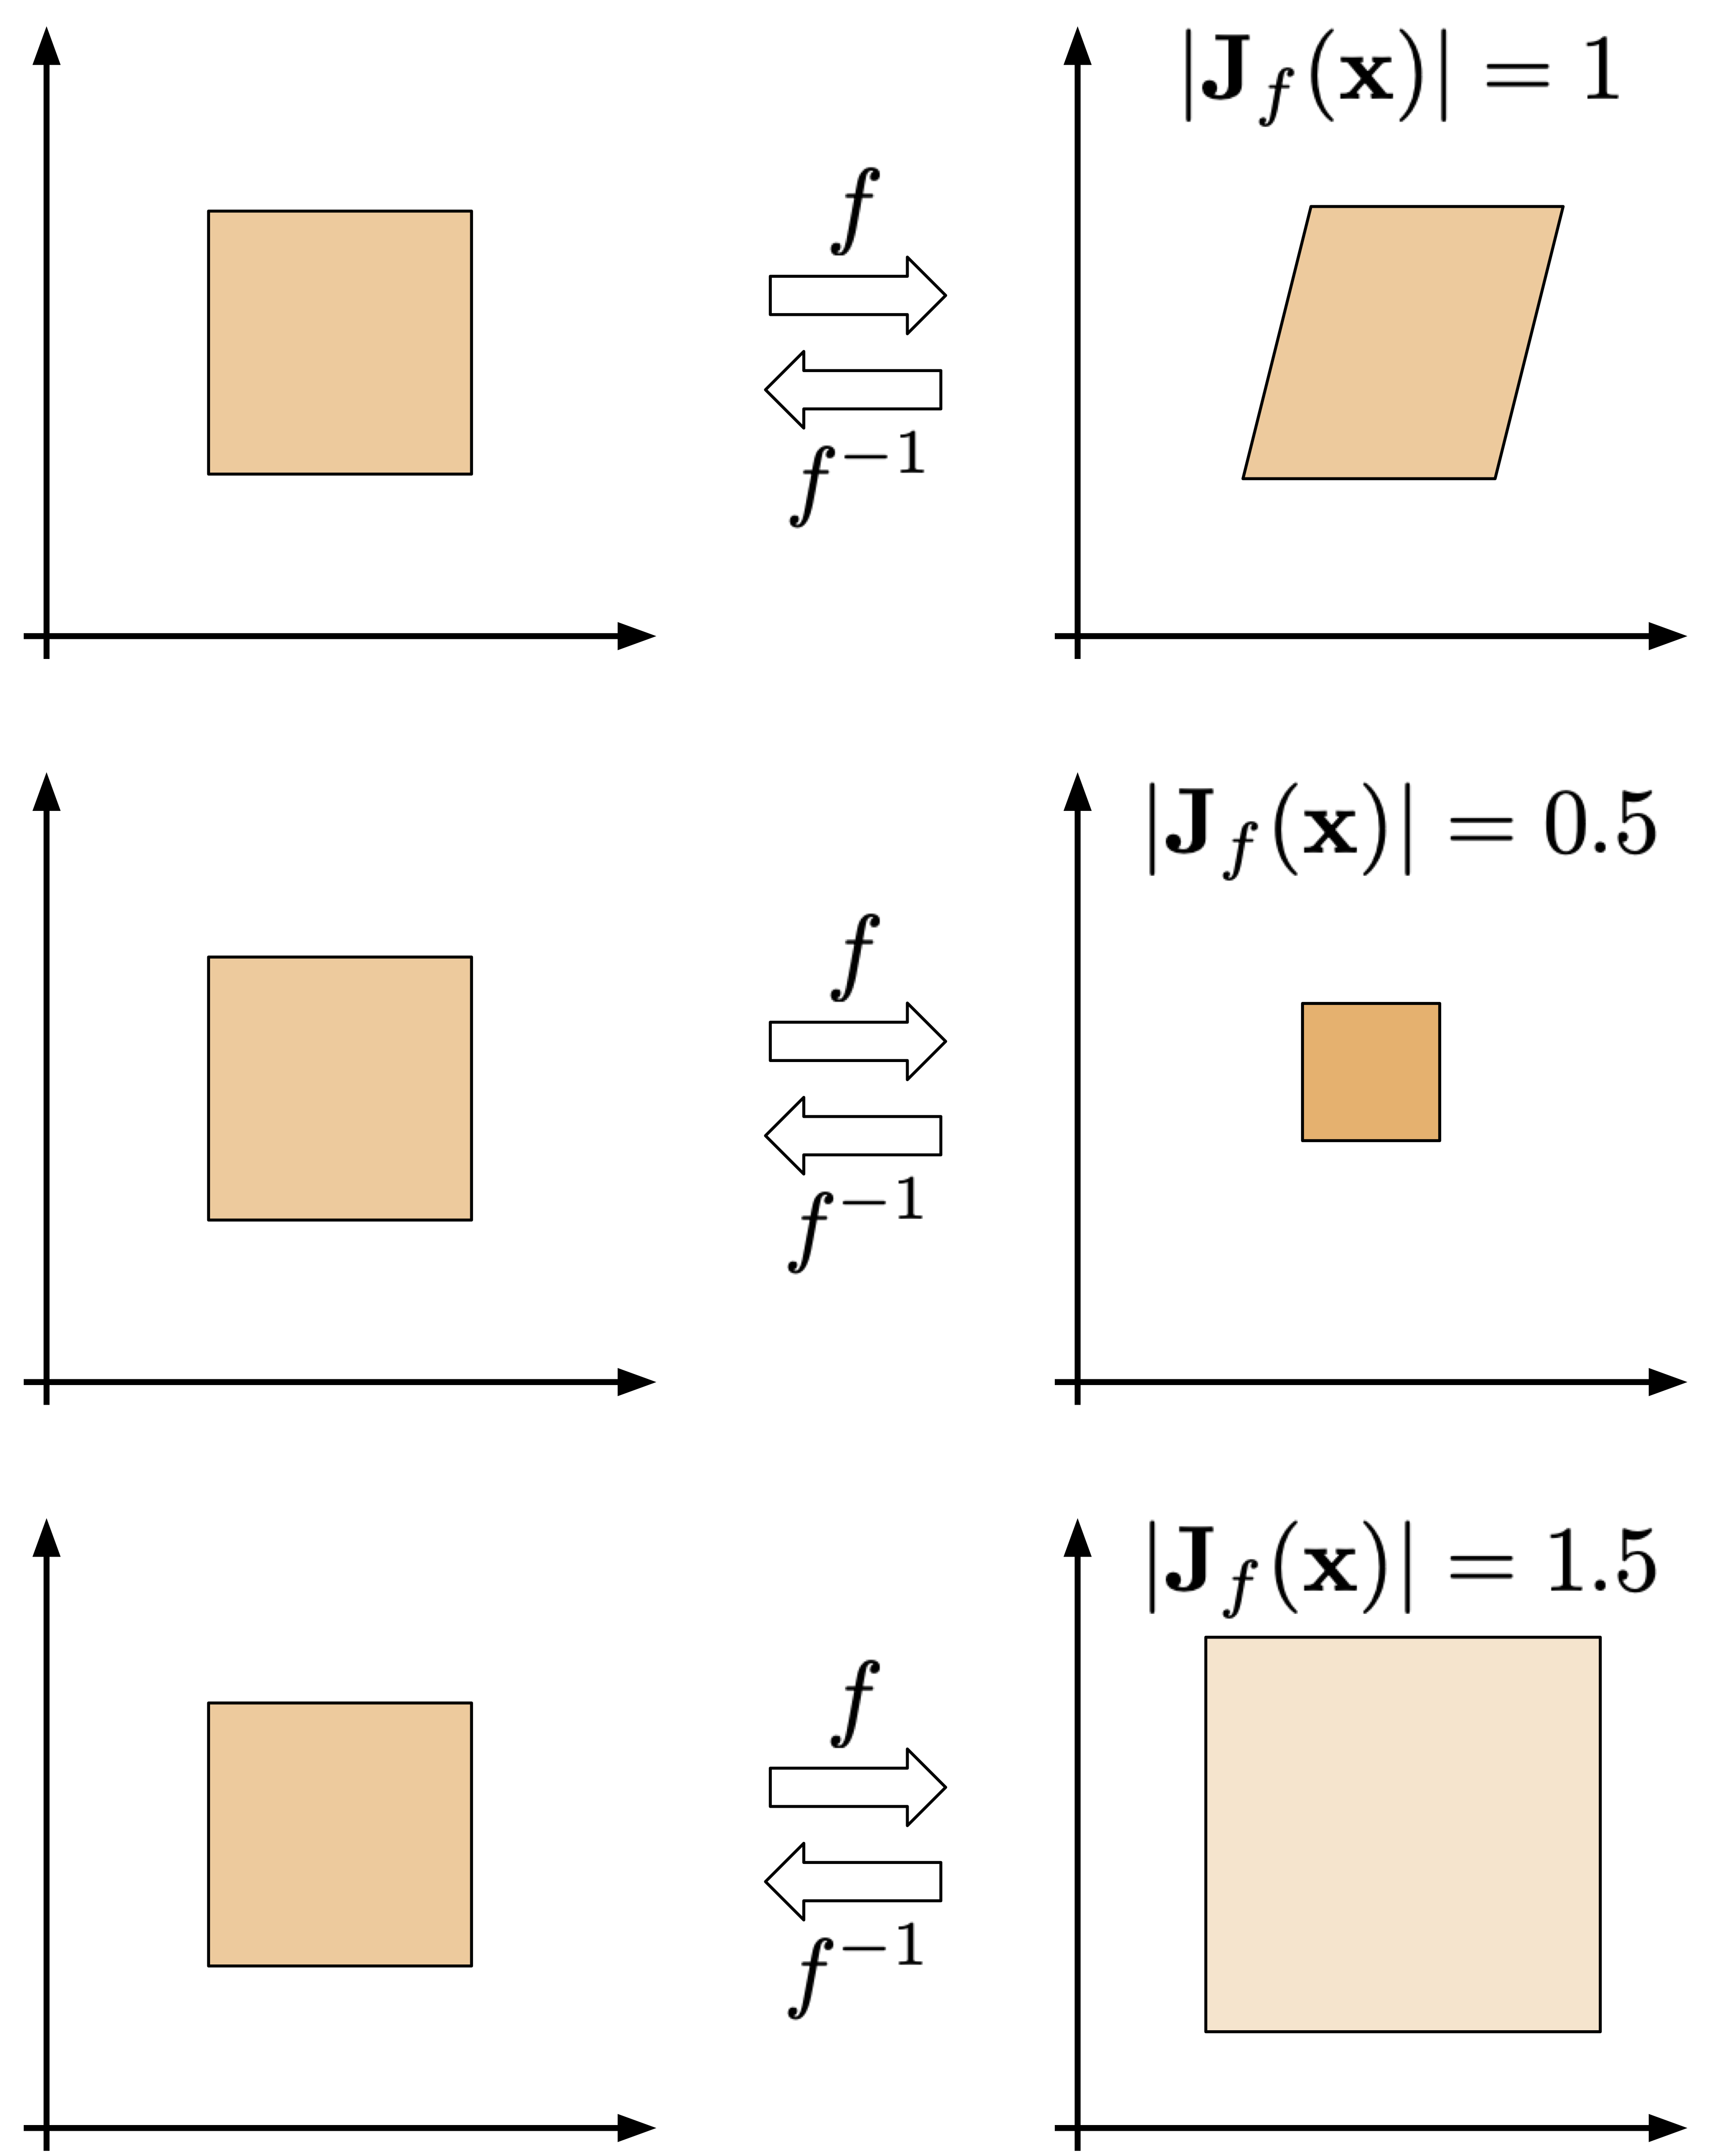
\includegraphics[width=\linewidth]{figs/jacobian_det}
		\end{figure}
	\end{minipage}
	\myfootnotewithlink{https://jmtomczak.github.io/blog/3/3\_flows.html}{https://jmtomczak.github.io/blog/3/3\_flows.html}
\end{frame}
%=======
\begin{frame}{Fitting flows}
	\begin{block}{MLE problem}
		\vspace{-0.3cm}
		\[
			p(\bx|\btheta) = p(\bz) \left|\det \left(  \frac{\partial \bz}{\partial \bx} \right) \right|  = p(f(\bx, \btheta)) \left|\det \left( \frac{\partial f(\bx, \btheta)}{\partial \bx} \right) \right|
		\]
		\[
			\log p(\bx|\btheta) = \log p(f(\bx, \btheta)) + \log  \left|\det \left( \frac{\partial f(\bx, \btheta)}{\partial \bx} \right) \right| \rightarrow \max_{\btheta}
		\]
	\end{block}
	\vspace{-0.2cm}
	\begin{figure}
		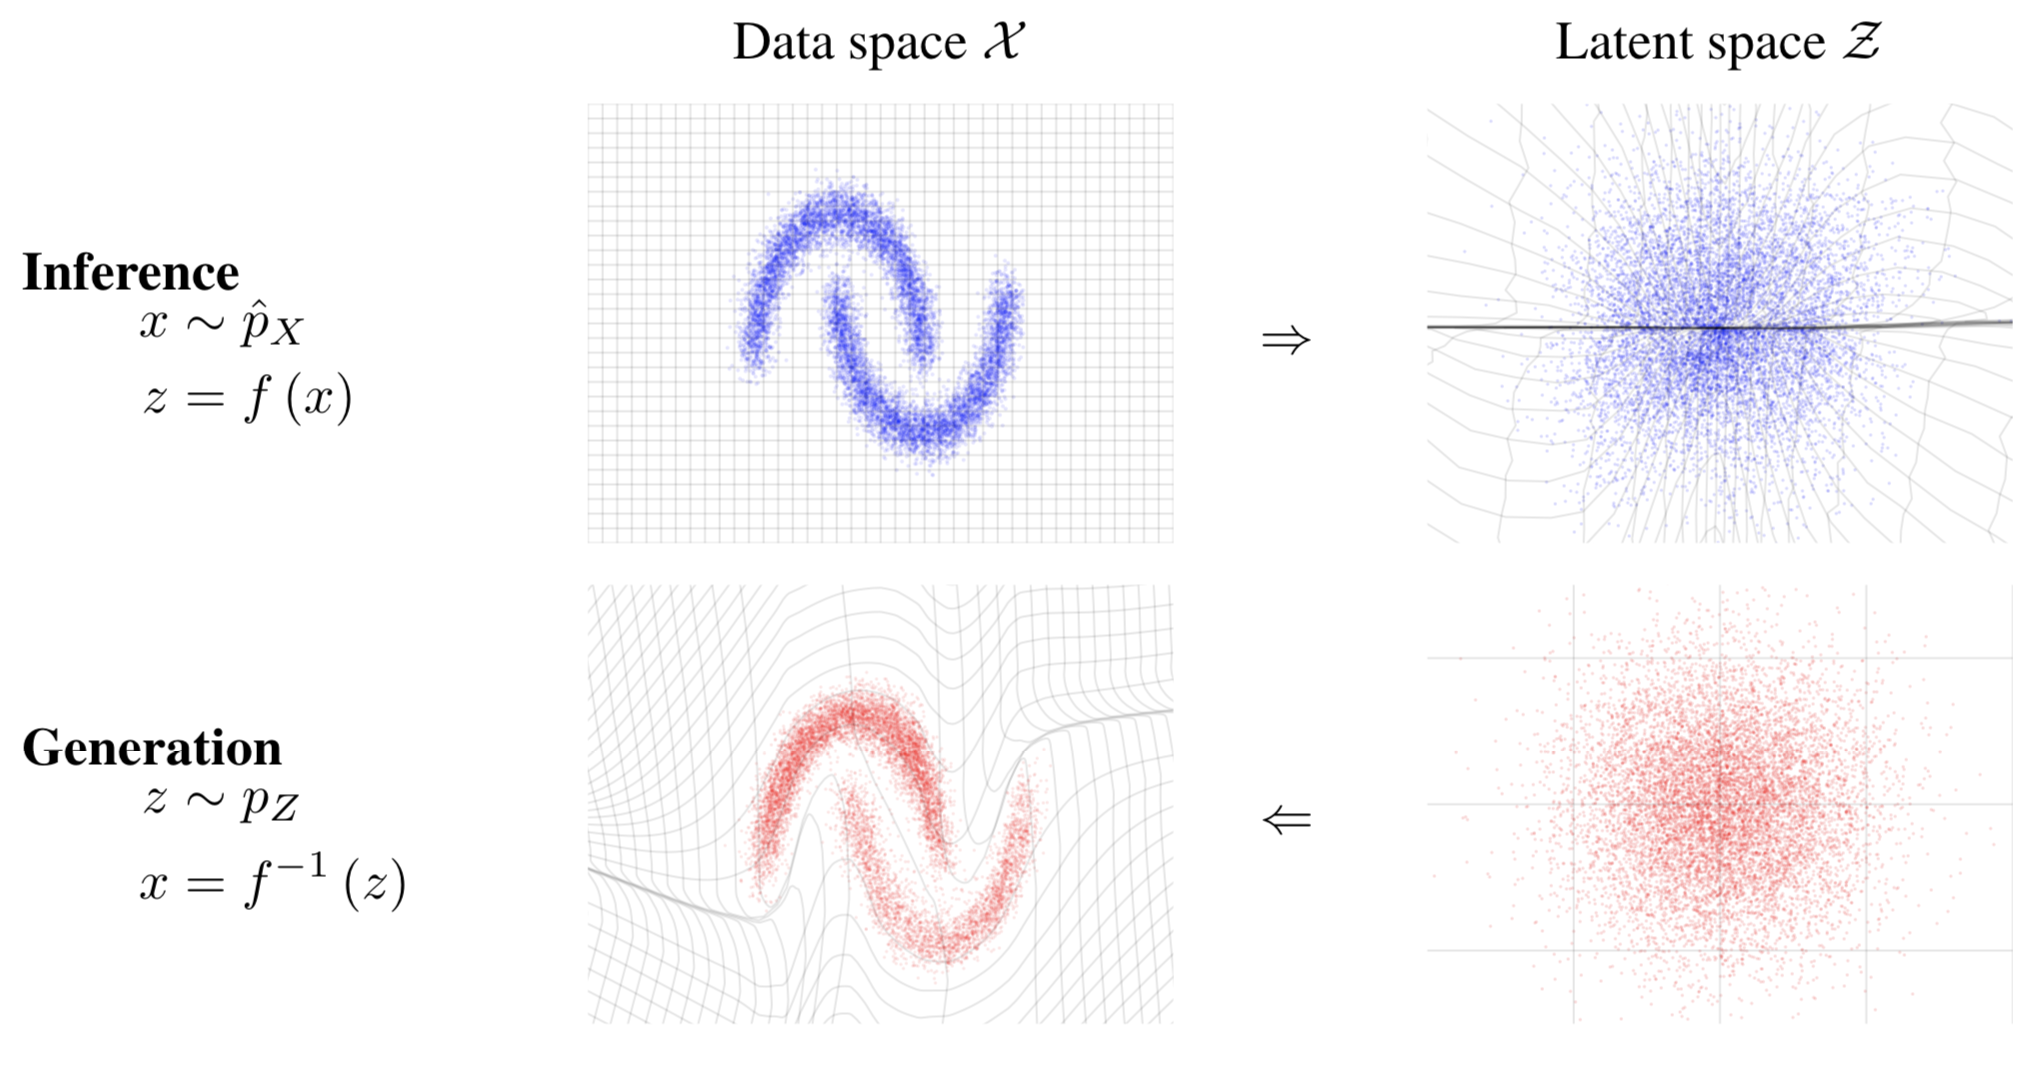
\includegraphics[width=0.85\linewidth]{figs/flows_how2}
	\end{figure}
	\myfootnotewithlink{https://arxiv.org/abs/1605.08803}{Dinh L., Sohl-Dickstein J., Bengio S. Density estimation using Real NVP, 2016} 
\end{frame}
%=======
\begin{frame}{Composition of flows}
	\begin{block}{Theorem}
		Diffeomorphisms are \textbf{composable} (If $\{f_k\}_{k=1}^K$ satisfy conditions of the change of variable theorem, then $\bz = f(\bx) = f_K \circ \dots \circ f_1(\bx)$ also satisfies it).
	\end{block}
	\vspace{-0.5cm}
	{ \footnotesize
	\begin{multline*}
		p(\bx) = p(f(\bx)) \left|\det \left(  \frac{\partial f(\bx)}{\partial \bx} \right) \right| = p(f(\bx)) \left|\det \left(\frac{\partial f_K \circ \dots \circ f_1(\bx)}{\partial \bx} \right) \right| = \\ =
		p(f(\bx)) \left|\det \left(\frac{\partial \textbf{f}_K}{\partial \textbf{f}_{K-1}} \dots \frac{\partial \textbf{f}_1}{\partial \bx} \right) \right| = p(f(\bx)) \prod_{k=1}^K \left|\det \left(\frac{\partial \textbf{f}_{k}}{\partial \textbf{f}_{k-1}} \right) \right|
	\end{multline*}
	}
	\vspace{-0.3cm}
	\begin{figure}
		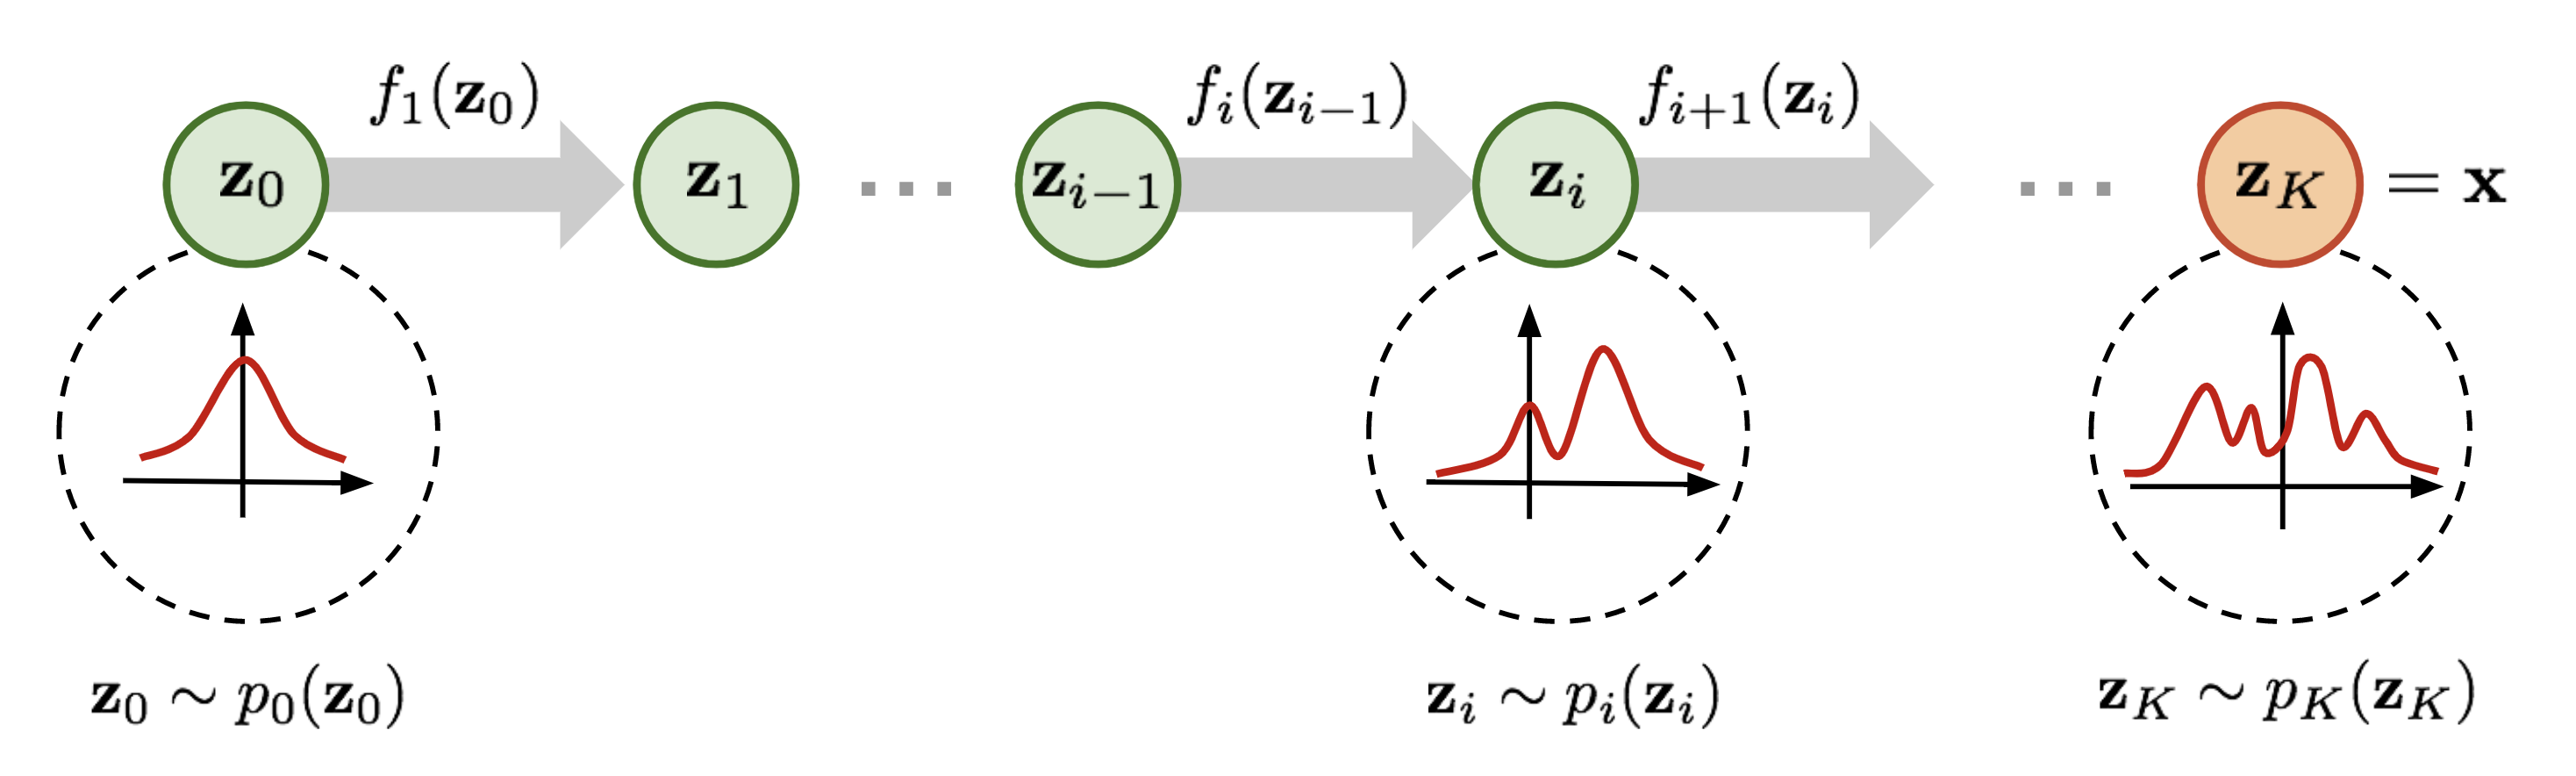
\includegraphics[width=\linewidth]{figs/normalizing-flow}
	\end{figure}
	\myfootnotewithlink{https://lilianweng.github.io/lil-log/2018/10/13/flow-based-deep-generative-models.html}{https://lilianweng.github.io/lil-log/2018/10/13/flow-based-deep-generative-models.html}
\end{frame}
%=======
\begin{frame}{Flows}
	\vspace{-0.3cm}
	\[
		\log p(\bx|\btheta) = \log p(f(\bx, \btheta)) + \log \left|\det \left( \frac{\partial f(\bx, \btheta)}{\partial \bx} \right) \right|
	\]
	\vspace{-0.3cm}
	\begin{block}{Definition}
		Normalizing flow is a \textit{differentiable, invertible} mapping from data $\bx$ to the noise $\bz$. 
	\end{block}
	\begin{itemize}
		\item \textbf{Normalizing} means that the inverse flow takes samples from $p(\bx)$ and normalizes them into samples from density $p(\bz)$.
		\item \textbf{Flow} refers to the trajectory followed by samples from $p(\bz)$ as they are transformed by the sequence of transformations
		\[
		\bz = f_K \circ \dots \circ f_1(\bx); \quad \bx = f_1^{-1} \circ \dots \circ f_K^{-1} (\bz) = g_1 \circ \dots \circ g_K(\bz) 
		\] 
		\begin{multline*}
			p(\bx) = p(f_K \circ \dots \circ f_1(\bx)) \left|\det \left(\frac{\partial f_K \circ \dots \circ f_1(\bx)}{\partial \bx} \right) \right| = \\
			= p(f_K \circ \dots \circ f_1(\bx)) \prod_{k=1}^K \left|\det \left(\frac{\partial \mathbf{f}_k}{\partial \mathbf{f}_{k-1}} \right) \right|.
		\end{multline*}
	\end{itemize}
\end{frame}
%=======
\begin{frame}{Flows}
	\begin{block}{Example of a 4-step flow}
	\vspace{-0.2cm}
	\begin{figure}
			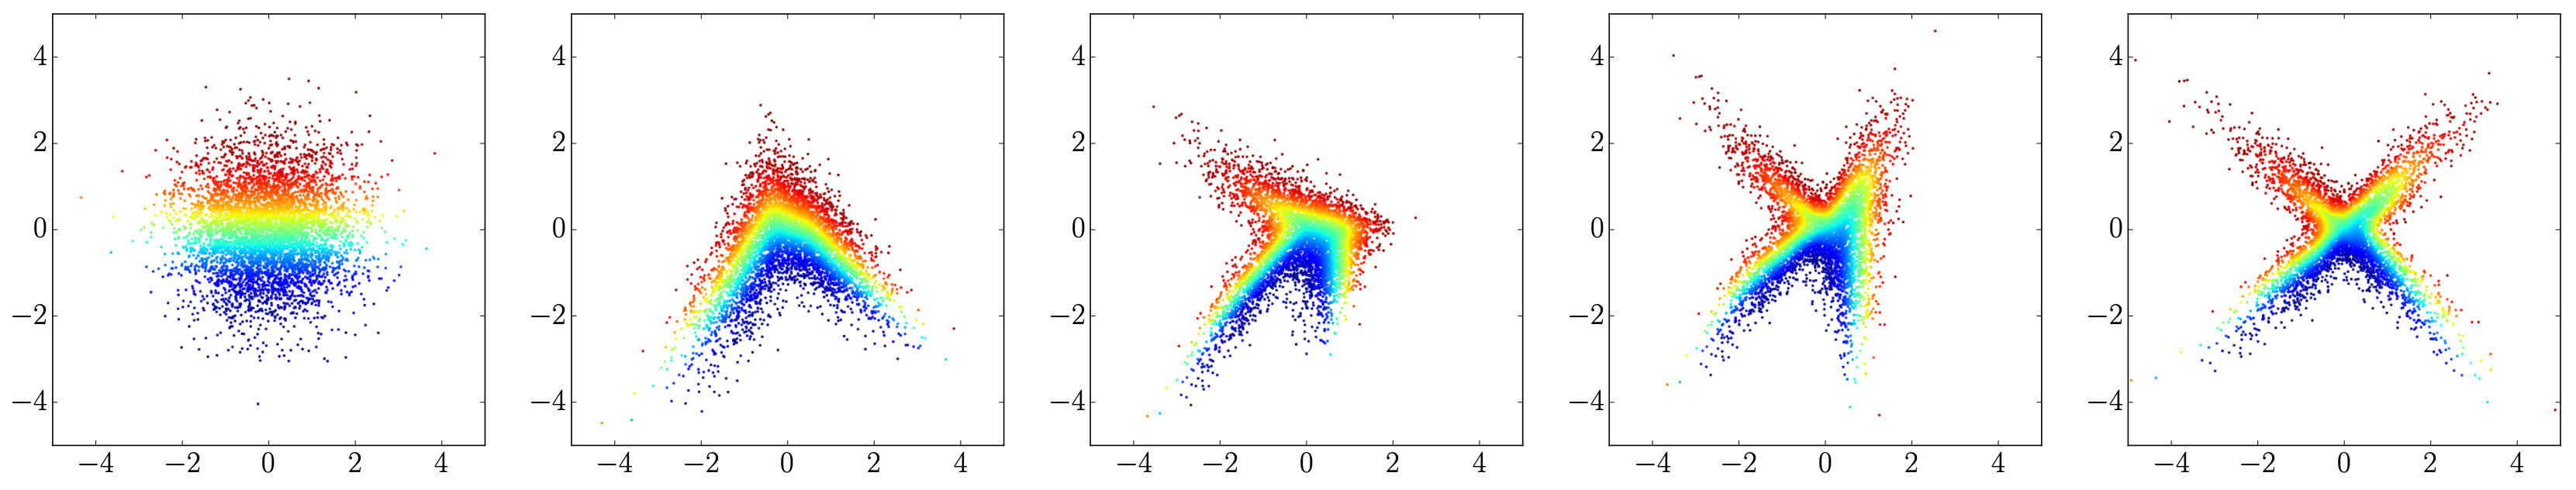
\includegraphics[width=\linewidth]{figs/flow_4_steps_example.png}
	\end{figure}
	\end{block}
	\vspace{-0.5cm}
	\begin{block}{Flow likelihood}
		\vspace{-0.3cm}
		\[
		\log p(\bx|\btheta) = \log p(f(\bx, \btheta)) + \log \left|\det \left( \frac{\partial f(\bx, \btheta)}{\partial \bx} \right) \right|
		\]
		\vspace{-0.3cm}
	\end{block}
	What is the complexity of the determinant computation?
	\begin{block}{What we want}
		\begin{itemize}
			\item Efficient computation of Jacobian $\frac{\partial f(\bx, \btheta)}{\partial \bx}$;
			\item Efficient sampling from the base distribution $p(\bz)$;
			\item Efficient inversion of $f(\bx, \btheta)$.
		\end{itemize}
	\end{block}
		\myfootnotewithlink{https://arxiv.org/abs/1912.02762}{Papamakarios G. et al. Normalizing flows for probabilistic modeling and inference, 2019} 
\end{frame}
%=======
\begin{frame}{Forward KL vs Reverse KL}
	\begin{block}{Forward KL}
		\vspace{-0.5cm}
		\begin{align*}
			KL(\pi || p) &= \int \pi (\bx) \log \frac{\pi(\bx)}{p(\bx | \btheta)} d \bx \\
			&= - \bbE_{\pi(\bx)} \log p(\bx | \btheta) + \text{const} \rightarrow \min_{\btheta}
		\end{align*}
		Maximum likelihood estimation is equivalent to minimization of the Monte-Carlo estimation of forward KL.
	\end{block}
	\begin{block}{Forward KL for flow model}
	    \vspace{-0.3cm}
		\[
			\log p(\bx|\btheta) = \log p(f(\bx, \btheta)) + \log  \left|\det \left( \frac{\partial f(\bx, \btheta)}{\partial \bx} \right) \right|
		\]
		\begin{itemize}
		\item We need to be able to compute $f(\bx, \btheta)$ and its Jacobian.
		\item We need to be able to compute the density $p(\bz)$.
		\item We don’t need to think about computing the function $g(\bz, \btheta) = f^{-1}(\bz, \btheta)$ until we want to sample from the flow.
		\end{itemize}
	\end{block}
\end{frame}
%=======
\begin{frame}{Forward KL vs Reverse KL}
	\begin{block}{Reverse KL}
	  	\vspace{-0.5cm}
			\begin{align*}
				KL(p || \pi) &= \int p(\bx | \btheta) \log \frac{p(\bx | \btheta)}{\pi(\bx)} d \bx \\
				&= \bbE_{p(\bx | \btheta)} \left[\log p(\bx | \btheta) - \log \pi(\bx)\right] \rightarrow \min_{\btheta}
			\end{align*}
		\vspace{-0.7cm}
	\end{block}
	\begin{block}{Reverse KL for flow model}
  		\vspace{-0.3cm}
		\[
			\log p(\bz) = \log p(\bx | \btheta) + \log \left|\det \left( \frac{\partial g(\bz, \btheta)}{\partial \bz} \right) \right|
		\]
		\[
			KL(p || \pi)  = \bbE_{p(\bz)} \left[  \log p(\bz) - \log \left|\det \left( \frac{\partial g(\bz, \btheta)}{\partial \bz} \right) \right| - \log \pi(g(\bz, \btheta)) \right]
		\]
		\begin{itemize}
		\item We need to be able to compute $g(\bz, \btheta)$ and its Jacobian.
		\item We need to be able to sample from the density $p(\bz)$ (do not need to evaluate it).
		\item We don’t need to think about computing the function $f(\bx, \btheta)$.
		\end{itemize}
	\end{block}
\end{frame}
%=======
\begin{frame}{Flow KL duality}
	\begin{block}{Theorem}
		Fitting flow model $p(\bx| \btheta)$ to the target distribution $\pi(\bx)$ using forward KL (MLE) is equivalent to fitting the induced distribution $p(\bz| \btheta)$ to the base $p(\bz)$ using reverse KL:
		\[
			\argmin_{\btheta} KL(\pi(\bx) || p(\bx | \btheta)) = \argmin_{\btheta} KL(p(\bz | \btheta) || p(\bz)).
		\]
		\vspace{-0.3cm}
		\begin{itemize}
			\item $p(\bz)$ is a base distribution; $\pi(\bx)$ is a data distribution;
			\item $\bz \sim p(\bz)$, $\bx = g(\bz, \btheta)$, $\bx \sim p(\bx| \btheta)$;
			\item $\bx \sim \pi(\bx)$, $\bz = f(\bx, \btheta)$, $\bz \sim p(\bz | \btheta)$;
		\end{itemize}
		\vspace{-0.3cm}
		\begin{align*}
			\log p(\bz | \btheta) &= \log \pi(g(\bz, \btheta)) + \log \left| \det \left( \frac{\partial g(\bz, \btheta)}{\partial \bz}\right) \right|; \\
			\log p(\bx | \btheta) &= \log p(f(\bx, \btheta)) + \log \left| \det \left( \frac{\partial f(\bx, \btheta)}{\partial \bx}\right) \right|.
		\end{align*}
	\end{block}
	\myfootnotewithlink{https://arxiv.org/abs/1912.02762}{Papamakarios G. et al. Normalizing flows for probabilistic modeling and inference, 2019} 
\end{frame}
%=======
\begin{frame}{Flow KL duality}
	\begin{block}{Theorem}
		Fitting flow model $p(\bx| \btheta)$ to the target distribution $\pi(\bx)$ using forward KL (MLE) is equivalent to fitting the induced distribution $p(\bz| \btheta)$ to the base $p(\bz)$ using reverse KL:
		\[
			\argmin_{\btheta} KL(\pi(\bx) || p(\bx | \btheta)) = \argmin_{\btheta} KL(p(\bz | \btheta) || p(\bz)).
		\]
		\vspace{-0.7cm}
	\end{block}
	\begin{block}{Proof}
		\vspace{-0.7cm}
		\begin{multline*}
			KL\left(p(\bz | \btheta) || \pi(\bz) \right) = \mathbb{E}_{p(\bz | \btheta)} \bigl[ \log p(\bz | \btheta) - \log p(\bz) \bigr] = \\ 
			= \mathbb{E}_{p(\bz | \btheta)} \left[ \log \pi(g(\bz, \btheta)) + \log \left| \det \left( \frac{\partial g(\bz, \btheta)}{\partial \bz}\right) \right| - \log p(\bz) \right] = \\
			= \mathbb{E}_{\pi(\bx)} \left[ \log \pi(\bx) - \log \left| \det \left( \frac{\partial f(\bx, \btheta)}{\partial \bx}\right) \right| - \log p(f(\bx, \btheta)) \right] = \\
			= \mathbb{E}_{\pi(\bx)} \bigl[ \log \pi(\bx) - \log p(\bx | \btheta) \bigr] = KL (\pi(\bx) || p(\bx | \btheta)).
		\end{multline*}
	\end{block}
	\myfootnotewithlink{https://arxiv.org/abs/1705.07057}{Papamakarios G., Pavlakou T., Murray I. Masked Autoregressive Flow for Density Estimation, 2017} 
\end{frame}
%=======
\begin{frame}{Jacobian structure}
	\begin{block}{Flow log-likelihood}
		\[
			\log p(\bx|\btheta) = \log p(f(\bx, \btheta)) + \log \left|\det \left( \frac{\partial f(\bx, \btheta)}{\partial \bx} \right) \right|
		\]
	\end{block}
	The main challenge is a determinant of the Jacobian.
	\begin{enumerate}
		\begin{block}{What is a det of Jacobian in the following cases?}
			\item Consider a linear layer $\bz = \bW \bx$.
			\item Let $\bz$ be a permutation of $\bx$. 
			\item Let $z_i$ depend only on $\bx_i$. 
			\[
				\log \left|\det \left( \frac{\partial f(\bx, \btheta)}{\partial \bx} \right) \right| = \log \left| \prod_{i=1}^m f_i'(x_i, \btheta) \right| = \sum_{i=1}^m \log \left| f_i'(x_i, \btheta) \right|.
			\]
			\item Let $z_i$ depend only on $\bx_{1:i}$ (autoregressive dependency). 
		\end{block}
	\end{enumerate}
\end{frame}
%=======
\begin{frame}{Residual Flows}
	\begin{block}{Matrix determinant lemma}
		\vspace{-0.5cm}
		\[
			\det \left( \bI_m + \bV \bW^T \right) = \det ( \bI_d + \bW^T \bV ), \quad \text{where } \bV, \bW \in \bbR^{m \times d}.
		\]
		\vspace{-0.5cm}
	\end{block}
	\begin{block}{Planar flow}
		\vspace{-0.2cm}
		\[
			\bx = g(\bz, \btheta) = \bz + \mathbf{u} \, \sigma(\bw^T\bz + b).
		\]
		\vspace{-0.3cm}
	\end{block}
	Here $\btheta = \{\bu, \bw, b\}$, $\sigma(\cdot)$ is a smooth element-wise non-linearity.
	{\small
	\[
		\left| \det \left( \frac{\partial g(\bz, \btheta)}{\partial \bz} \right)\right| = \left| \det \left( \bI + \sigma'(\bw^T \bz + b) \bw\bu^T\right) \right| = \left| 1 + \sigma'(\bw^T \bz + b) \bw^T \bu \right|
	\]}
	The transformation is invertible, for example, if
	\[
		\sigma = \tanh; \quad \sigma'(\bw^T \bz + b) \bu^T \bw \geq -1.
	\]
	\myfootnotewithlink{https://arxiv.org/abs/1505.05770}{Rezende D. J., Mohamed S. Variational Inference with Normalizing Flows, 2015} 
\end{frame}
%=======
\begin{frame}{Residual Flows}
	\begin{block}{Expressiveness of planar flows}
		\vspace{-0.5cm}
		\[
			\bz_K = g_1 \circ \dots \circ g_K (\bz); \quad g_k = g(\bz_k, \btheta_k) = \bz_k + \bu_k\, \sigma(\bw_k^T\bz_k + b_k).
		\]
		\vspace{-0.8cm}
		\begin{figure}
			\centering
			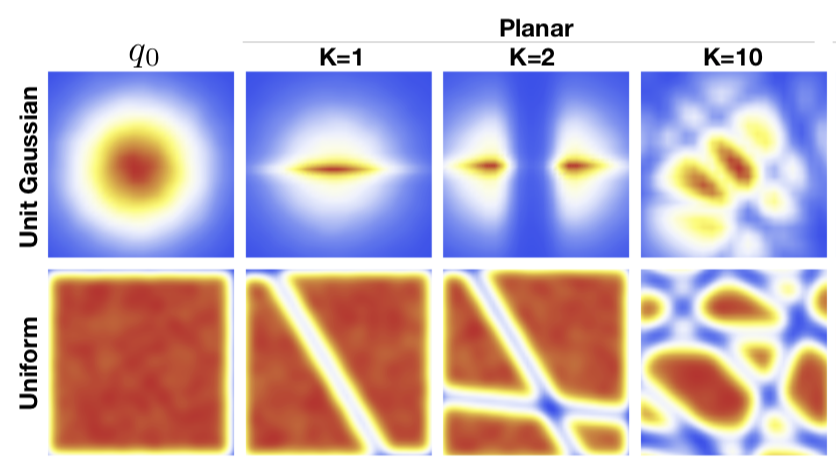
\includegraphics[width=0.7\linewidth]{figs/planar_flows.png}
		\end{figure}
		\vspace{-0.5cm}
	\end{block}
	\begin{block}{Sylvester flow: planar flow extension}
		\vspace{-0.3cm}
		\[
		g(\bz, \btheta) = \bz + \bV \, \sigma(\bW^T\bz + \mathbf{b}).
		\]
	\end{block}
	\myfootnote{\href{https://arxiv.org/abs/1505.05770}{Rezende D. J., Mohamed S. Variational Inference with Normalizing Flows, 2015}\\
	\href{https://arxiv.org/abs/1803.05649}{Berg R. et al. Sylvester normalizing flows for variational inference, 2018}}
\end{frame}
%=======
\begin{frame}{Linear flows}
	
	\begin{block}{RealNVP}
		\vspace{-0.5cm}
		\begin{equation*}
			\begin{cases} \bz_{1:d} = \bx_{1:d}; \\ \bz_{d:m} = \tau (\bx_{d:m}, c(\bx_{1:d}));\end{cases} 
			\quad \Leftrightarrow \quad 
			\begin{cases} \bx_{1:d} = \bz_{1:d}; \\ \bx_{d:m} = \tau^{-1} (\bz_{d:m}, c(\bz_{1:d})).\end{cases}
		\end{equation*}
		\vspace{-0.2cm}
	\end{block}
	\begin{itemize}
	\item First step is a \textbf{split} operator which decouples a variable into 2 subparts: $\bx_1$ and $\bx_2$ (usualy channel-wise).
	\item We should \textbf{permute} components between different layers.
	\end{itemize}
	\[
		\bz = \bW \bx, \quad \bW \in \bbR^{m \times m}
	\]
	In general, we need $O(m^3)$ to invert matrix.
	\begin{block}{Invertibility}
		\begin{itemize}
			\item Diagonal matrix $O(m)$.
			\item Triangular matrix $O(m^2)$.
			\item It is impossible to parametrize all invertible matrices.
		\end{itemize}
	\end{block}
\end{frame}
%=======
\begin{frame}{Linear flows}
	\vspace{-0.3cm}
	\[
		\bz = \bW \bx, \quad \bW \in \bbR^{m \times m}
	\]
	\vspace{-0.3cm}
	\begin{block}{Matrix decompositions}
		\begin{itemize}
			\item LU-decomposition
			\[
				\bW = \mathbf{P} \bL \bU,
			\]
			where $\mathbf{P}$ is a permutation matrix, $\mathbf{L}$ is lower triangular with positive diagonal, $\mathbf{U}$ is upper triangular with positive diagonal.
			\item QR-decomposition
			\[
				\bW = \bQ \mathbf{R},
			\]
			where $\bQ$ is an orthogonal matrix, $\mathbf{R}$ is an upper triangular matrix with positive diagonal.
		\end{itemize}
	\end{block}

	\myfootnote{
		\href{https://arxiv.org/abs/1807.03039}{Kingma D. P., Dhariwal P. Glow: Generative Flow with Invertible 1x1 Convolutions, 2018}  \\
		\href{https://arxiv.org/abs/1901.11137}{Hoogeboom E., Van Den Berg R., and Welling M. Emerging convolutions for generative normalizing flows, 2019}
	}
\end{frame}
%=======
\begin{frame}{Glow samples}
	\begin{figure}
		\centering
		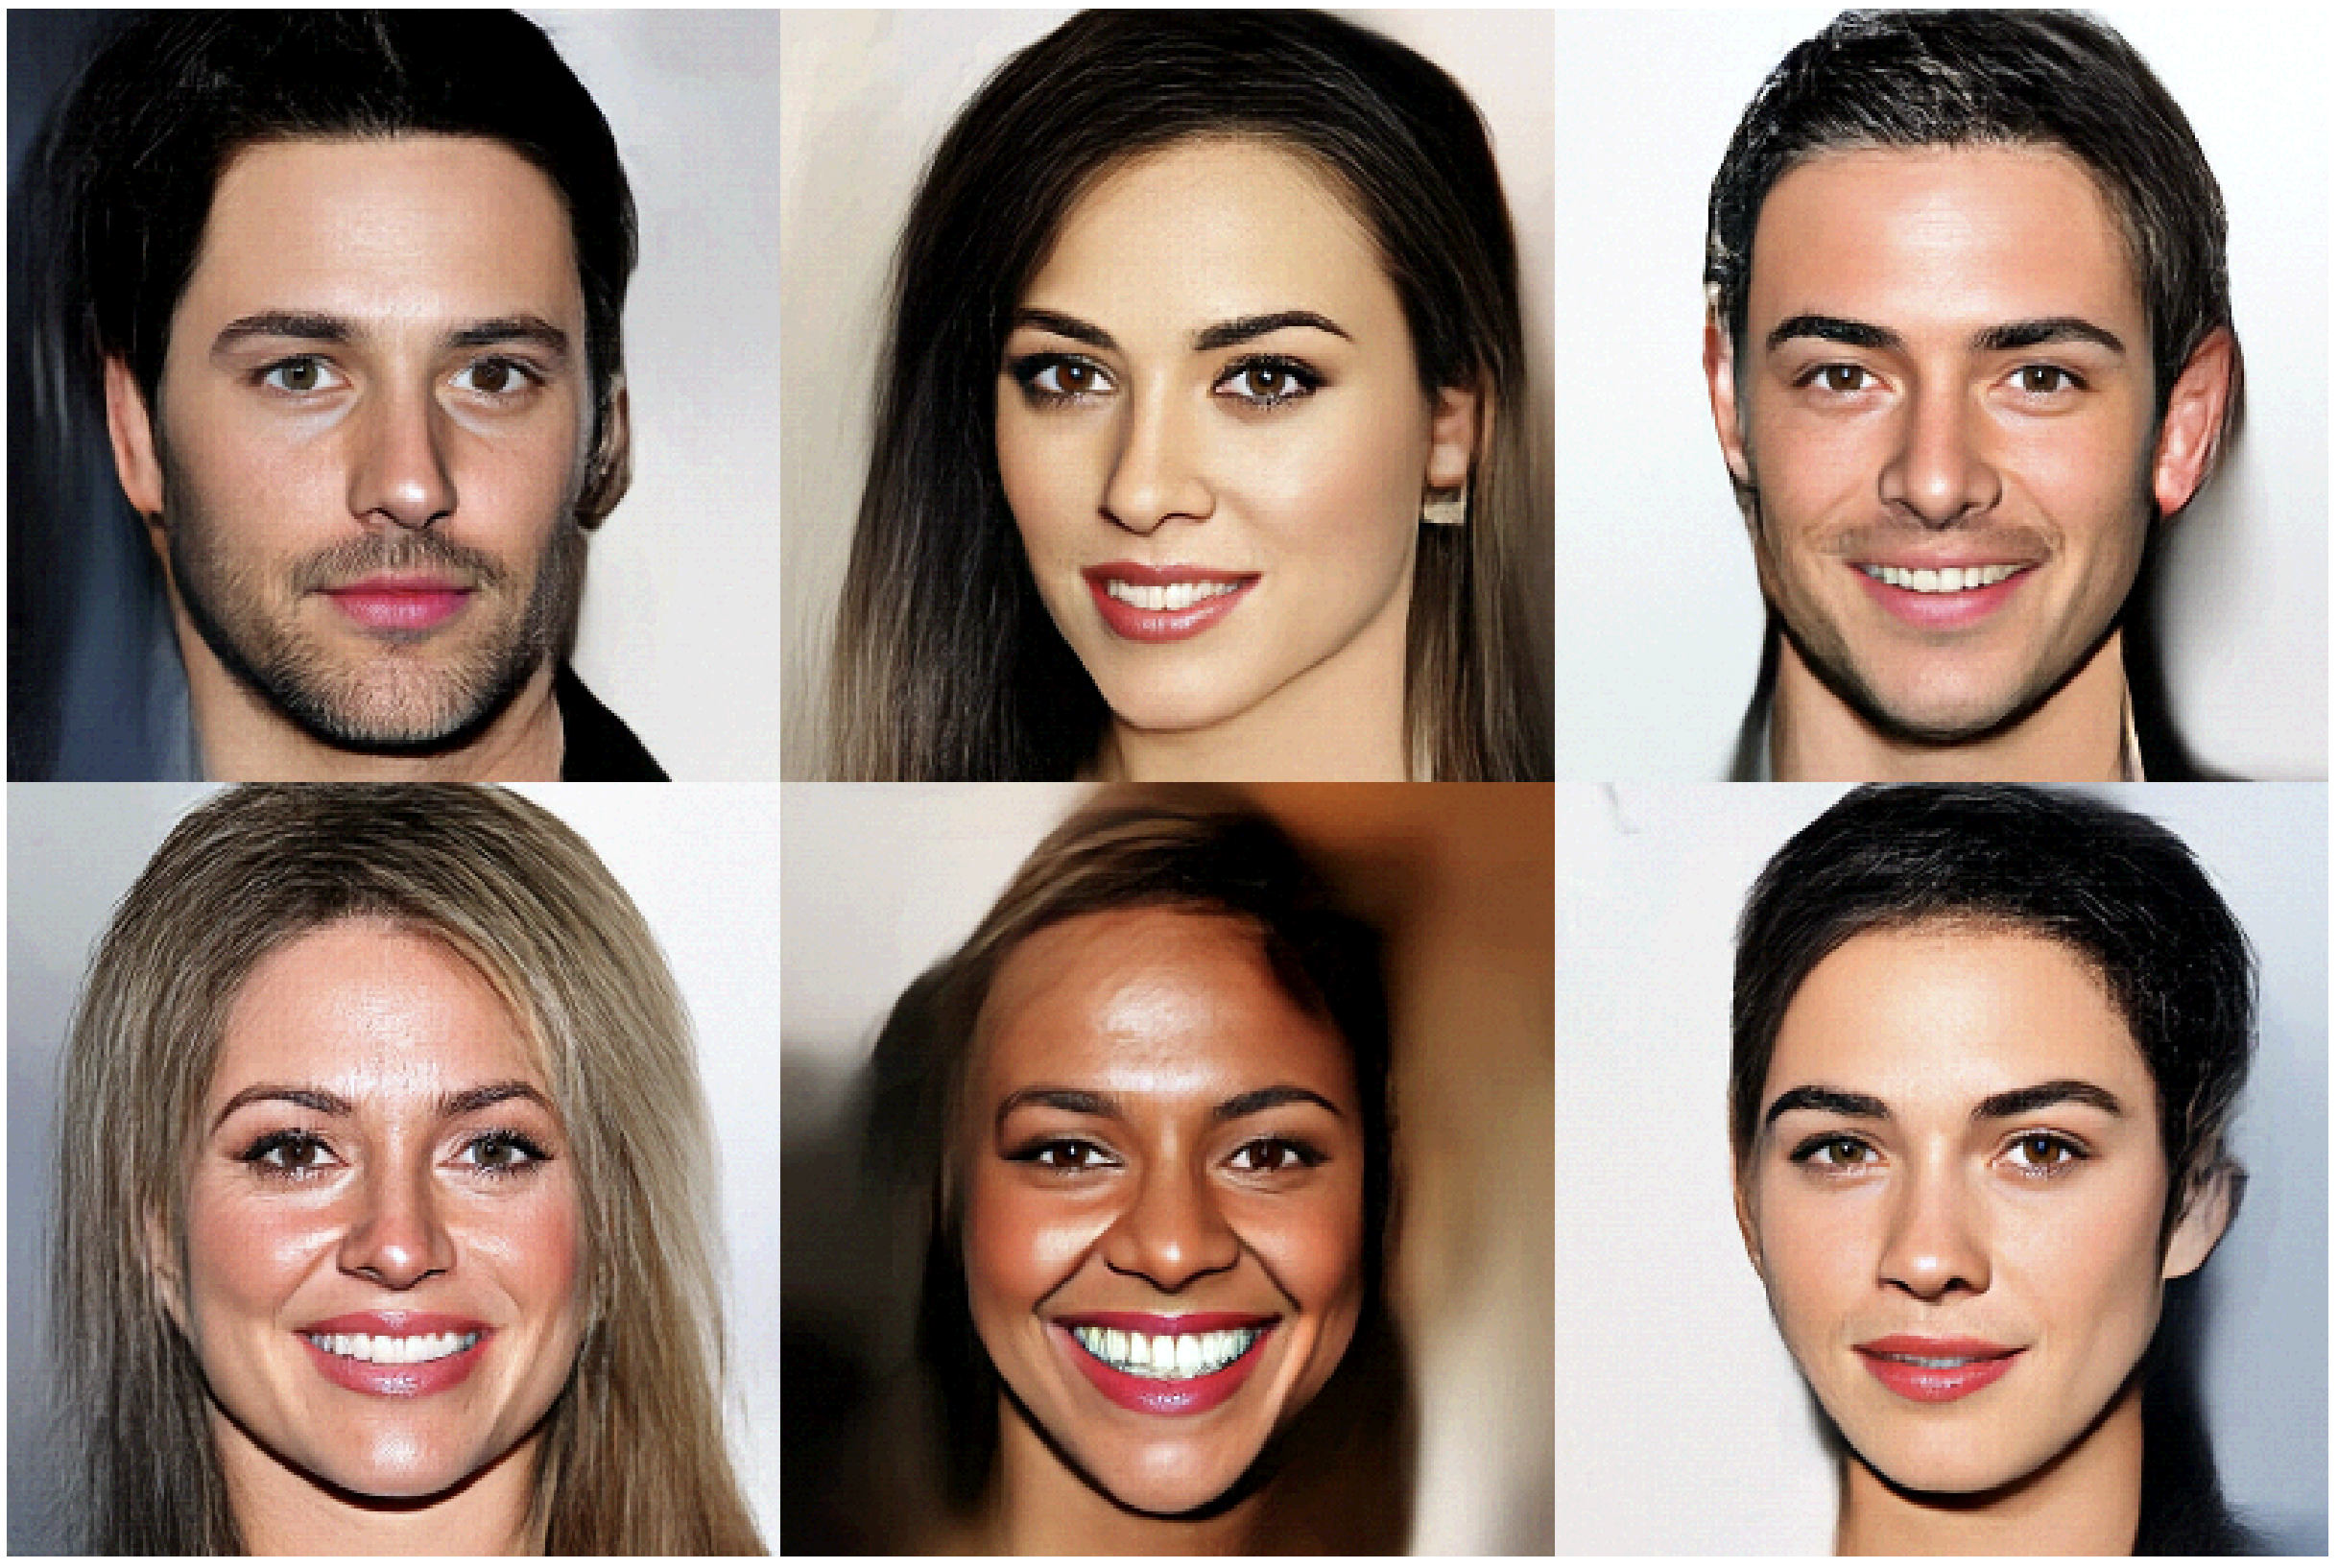
\includegraphics[width=\linewidth]{figs/glow_faces.png}
	\end{figure}
	\myfootnotewithlink{https://arxiv.org/abs/1807.03039}{Kingma D. P., Dhariwal P. Glow: Generative Flow with Invertible 1x1 Convolutions, 2018}
\end{frame}
%=======
\begin{frame}{Summary}
	\begin{itemize}
		\item Flow models transform a simple base distribution to a complex one via a sequence of invertible transformations with tractable Jacobian.
		\vfill
		\item Flow models have a tractable likelihood that is given by the change of variable theorem.
		\vfill
		\item Flows could be fitted using forward and reverse KL minimization. We will consider each of the scenarios later in the course.
		\vfill
		\item Planar and Sylvester flows are residual flows which use matrix determinant lemma. 
		\vfill 
		\item Linear flows try to parametrize set of invertible matrices via matrix decompositions.
	\end{itemize}
\end{frame}
\end{document} 